\RequirePackage[l2tabu, orthodox]{nag}
\RequirePackage{silence}
\WarningFilter{nag}{There is no environment ``centering'' }%nag complains because beamer titlepage uses a centering environment
\WarningFilter{nag}{1 complaints in total}
\WarningFilter{ifpdf}{Someone has redefined \pdfoutput}
\WarningFilter{fmtcount}{\ordinal already defined use \FCordinal instead}
\documentclass[english, french]{beamer}
%INSTALL

%avoids a warning
\usepackage[log-declarations=false]{xparse}
\usepackage{fontspec} %font selecting commands
\usepackage{xunicode}
%warn about missing characters
\tracinglostchars=2

%REDAC
\usepackage{booktabs}
\usepackage{calc}

\usepackage{mathtools} %load this before babel!
	\mathtoolsset{showonlyrefs,showmanualtags}

\usepackage{babel}
%suppresses the warning about frenchb not modifying the captions (“—” to “:” in “Figure 1 – Legend”).
	\frenchbsetup{AutoSpacePunctuation=false,SuppressWarning=false}

\usepackage[super]{nth}
\usepackage{listings} %typeset source code listings
	\lstset{language=XML,tabsize=2,literate={"}{{\tt"}}1,captionpos=b}
\usepackage[nolist,smaller,printonlyused]{acronym}%,smaller option produces warnings from relsize in some cases, it seems.
\usepackage[nodayofweek]{datetime}%must be loaded after the babel package
\usepackage{xspace}
\usepackage{hyperref}% option pdfusetitle must be introduced here, not in hypersetup.
%breaklinks makes links on multiple lines into different PDF links to the same target.
%colorlinks (false): Colors the text of links and anchors. The colors chosen depend on the the type of link. In spite of colored boxes, the colored text remains when printing.
%linkcolor=black: this leaves other links in colors, e.g. refs in green, don't print well.
%pdfborder (0 0 1, set to 0 0 0 if colorlinks): width of PDF link border
%hidelinks
\hypersetup{breaklinks,bookmarksopen,colorlinks=true,urlcolor=blue,linkcolor=,hyperfigures=true}
% hyperref doc says: Package bookmark replaces hyperref’s bookmark organization by a new algorithm (...) Therefore I recommend using this package.
\usepackage{bookmark}

% center floats by default, but do not use with float
% \usepackage{floatrow}
% \makeatletter
% \g@addto@macro\@floatboxreset\centering
% \makeatother
\usepackage{ragged2e} %new com­mands \Cen­ter­ing, \RaggedLeft, and \RaggedRight and new en­vi­ron­ments Cen­ter, FlushLeft, and FlushRight, which set ragged text and are eas­ily con­fig­urable to al­low hy­phen­ation (the cor­re­spond­ing com­mands in LaTeX, all of whose names are lower-case, pre­vent hy­phen­ation al­to­gether). 
\usepackage{siunitx} %[expproduct=tighttimes, decimalsymbol=comma]
\sisetup{detect-all}% to detect e.g. when in math mode (use a math font)
\usepackage{braket} %for \Set
\usepackage{natbib}

\usepackage{amsmath,amsthm}
% \usepackage{amsfonts} %not required?
% \usepackage{dsfont} %for what?
%unicode-math overwrites the following commands from the mathtools package: \dblcolon, \coloneqq, \Coloneqq, \eqqcolon. Using the other colon-like commands from mathtools will lead to inconsistencies. Plus, Using \overbracket and \underbracke from mathtools package. Use \Uoverbracket and \Uunderbracke for original unicode-math definition.
%use exclusively \mathbf and choose math bold style below.
\usepackage[warnings-off={mathtools-colon, mathtools-overbracket}, bold-style=ISO]{unicode-math}

\defaultfontfeatures{
	Fractions=On,
	Mapping=tex-text% to turn "--" into dashes, useful for bibtex%%
}
\defaultfontfeatures[\rmfamily, \sffamily]{
	Fractions=On,
	Mapping=% to leave " alone (disable the default mapping tex-text; requires loading the font afterwards?)
}
\newfontfamily\xitsfamily{XITS}
\newfontfamily\texgyretermesfamily{TeX Gyre Termes}
\newfontfamily\texgyreherosfamily{TeX Gyre Heros}
\newfontfamily\lmfamily{Latin Modern Roman}
\setmainfont{Latin Modern Roman}
\setsansfont{Latin Modern Sans}
\setmonofont{Latin Modern Mono}
\defaultfontfeatures{}%disable default font features to avoid warnings with math fonts.
\setmathfont{XITS Math}
\setmathfont[range={\mathcal,\mathbfcal},StylisticSet=1]{XITS Math}

\usepackage{cleveref}% cleveref should go "laster" than hyperref
%GRAPHICS
\usepackage{pgf}
\usepackage{pgfplots}
	\usetikzlibrary{matrix,fit,plotmarks,calc,trees,shapes.geometric,positioning,plothandlers}
\pgfplotsset{compat=1.11}
\usepackage{graphicx}

\graphicspath{{graphics/},{graphics-dm/}}
\DeclareGraphicsExtensions{.pdf}

%HACKING
\usepackage{printlen}
\uselengthunit{mm}
% 	\newlength{\templ}% or LenTemp?
% 	\setlength{\templ}{6 pt}
% 	\printlength{\templ}
\usepackage{etoolbox} %for addtocmd command
\usepackage{scrhack}% load at end. Corrects a bug in float package, which is outdated but might be used by other packages
\usepackage{xltxtra} %somebody said that this is loaded by fontspec, but does not seem correct: if not loaded explicitly, does not appear in the log and \showhyphens is not corrected.

%Beamer-specific
%ADD
\usepackage{appendixnumberbeamer}
%\setbeamersize{text margin left=0.1cm, text margin right=0.1cm} 
\setbeamertemplate{navigation symbols}{}
\usetheme{BrusselsBelgium}
\usefonttheme{professionalfonts}


\newcommand{\R}{ℝ}
\newcommand{\N}{ℕ}
\newcommand{\Z}{ℤ}
\newcommand{\card}[1]{\lvert{#1}\rvert}
\newcommand{\powerset}[1]{\mathscr{P}(#1)}%\mathscr rather than \mathcal: scr is rounder than cal (at least in XITS Math).
\newcommand{\suchthat}{\;\ifnum\currentgrouptype=16 \middle\fi|\;}
%\newcommand{\Rplus}{\reels^+\xspace}

\AtBeginDocument{%
	\renewcommand{\epsilon}{\varepsilon}
% we want straight form of \phi for mathematics, as recommended in UTR #25: Unicode support for mathematics.
%	\renewcommand{\phi}{\varphi}
}

% with amssymb, but I don’t want to use amssymb just for that.
% \newcommand{\restr}[2]{{#1}_{\restriction #2}}
%\newcommand{\restr}[2]{{#1\upharpoonright}_{#2}}
\newcommand{\restr}[2]{{#1|}_{#2}}%sometimes typed out incorrectly within \set.
%\newcommand{\restr}[2]{{#1}_{\vert #2}}%\vert errors when used within \Set and is typed out incorrectly within \set.
\DeclareMathOperator*{\argmax}{arg\,max}
\DeclareMathOperator*{\argmin}{arg\,min}


%ARG TH
\newcommand{\AF}{\mathcal{AF}}
\newcommand{\labelling}{\mathcal{L}}
\newcommand{\labin}{\textbf{in}\xspace}
\newcommand{\labout}{\textbf{out}}
\newcommand{\labund}{\textbf{undec}\xspace}
\newcommand{\nonemptyor}[2]{\ifthenelse{\equal{#1}{}}{#2}{#1}}
\newcommand{\gextlab}[2][]{
	\labelling{\mathcal{GE}}_{(#2, \nonemptyor{#1}{\ibeatsr{#2}})}
}
\newcommand{\allargs}{A^*}
\newcommand{\args}{A}
\newcommand{\ar}{a}

%MCDA+Arg
\newcommand{\dm}{d}
\newcommand{\ileadsto}{\leadsto}
\newcommand{\mleadsto}[1][\eta]{\leadsto_{#1}}
\newcommand{\ibeats}{\vartriangleright}
\newcommand{\mbeats}[1][\eta]{\vartriangleright_{#1}}


%MISC
\newcommand{\lequiv}{\Vvdash}
\newcommand{\weightst}{W^{\,t}}

%MCDA classical
\newcommand{\crits}{\mathcal{J}}
\newcommand{\altspace}{\mathbb{A}}
\newcommand{\alts}{A}

%Sorting
\newcommand{\cats}{\mathcal{C}}
\newcommand{\catssubsets}{2^\cats}
\newcommand{\catgg}{\vartriangleright}
\newcommand{\catll}{\vartriangleleft}
\newcommand{\catleq}{\trianglelefteq}
\newcommand{\catgeq}{\trianglerighteq}
\newcommand{\alttoc}[2][x]{(#1 \xrightarrow{} #2)}
\newcommand{\alttocat}[3]{(#2 \xrightarrow{#1} #3)}
\newcommand{\alttoI}{(x \xrightarrow{} \left[\underline{C_x}, \overline{C_x}\right])}
\newcommand{\alttocatdm}[3][t]{\left(#2 \thinspace \raisebox{-3pt}{$\xrightarrow{#1}$}\thinspace #3\right)}
\newcommand{\alttocatatleast}[2]{\left(#1 \thinspace \raisebox{-3pt}{$\xrightarrow[]{≥}$}\thinspace #2\right)}
\newcommand{\alttocatatmost}[2]{\left(#1 \thinspace \raisebox{-3pt}{$\xrightarrow[]{≤}$}\thinspace #2\right)}

\newcommand{\source}{\scriptsize}
\newcommand{\commentOC}[1]{{\selectlanguage{french}{\todo{OC : #1}}}}
%Or: \todo[color=green!40]

%this probably requires outdated float package, see doc KomaScript for an alternative.
% \newfloat{program}{t}{lop}
% \floatname{program}{PM}

%\crefname{axiom}{axiom}{axioms}%might be needed for workaround bug in cref when defining new theorems?

%\ifdefined\theorem\else
%\newtheorem{theorem}{\iflanguage{english}{Theorem}{Théorème}}
%\fi

%which line breaks are chosen: accept worse lines, therefore reducing risk of overfull lines. Default = 200
\tolerance=2000
%accept overfull hbox up to...
\hfuzz=2cm
%reduces verbosity about the bad line breaks
\hbadness 5000
%sloppy sets tolerance to 9999
\apptocmd{\sloppy}{\hbadness 10000\relax}{}{}

% WRITING
%\newcommand{\ie}{i.e.\@\xspace}%to try
%\newcommand{\eg}{e.g.\@\xspace}
%\newcommand{\etal}{et al.\@\xspace}
\newcommand{\ie}{i.e.\ }
\newcommand{\eg}{e.g.\ }
\newcommand{\mkkOK}{\checkmark}%\color{green}{\checkmark}
\newcommand{\mkkREQ}{\ding{53}}%requires pifont?%\color{green}{\checkmark}
\newcommand{\mkkNO}{}%\text{\color{red}{\textsf{X}}}

\makeatletter
\newcommand{\boldor}[2]{%
	\ifnum\strcmp{\f@series}{bx}=\z@
		#1%
	\else
		#2%
	\fi
}
\newcommand{\textstyleElProm}[1]{\boldor{\MakeUppercase{#1}}{\textsc{#1}}}
\makeatother
\newcommand{\electre}{\textstyleElProm{Électre}\xspace}
\newcommand{\electreIv}{\textstyleElProm{Électre Iv}\xspace}
\newcommand{\electreIV}{\textstyleElProm{Électre IV}\xspace}
\newcommand{\electreIII}{\textstyleElProm{Électre III}\xspace}
\newcommand{\electreTRI}{\textstyleElProm{Électre Tri}\xspace}
% \newcommand{\utadis}{\texorpdfstring{\textstyleElProm{utadis}\xspace}{UTADIS}}
% \newcommand{\utadisI}{\texorpdfstring{\textstyleElProm{utadis i}\xspace}{UTADIS I}}

%TODO
% \newcommand{\textstyleElProm}[1]{{\rmfamily\textsc{#1}}} 


\newlength{\GraphsNodeSep}
\setlength{\GraphsNodeSep}{7mm}

% MCDA Drawing Sorting
\newlength{\MCDSCatHeight}
\setlength{\MCDSCatHeight}{6mm}
\newlength{\MCDSAltHeight}
\setlength{\MCDSAltHeight}{4mm}
%separation between two vertical alts
\newlength{\MCDSAltSep}
\setlength{\MCDSAltSep}{2mm}
\newlength{\MCDSCatWidth}
\setlength{\MCDSCatWidth}{3cm}
\newlength{\MCDSEvalRowHeight}
\setlength{\MCDSEvalRowHeight}{6mm}
\newlength{\MCDSAltsToCatsSep}
\setlength{\MCDSAltsToCatsSep}{1.5cm}
\newcounter{MCDSNbAlts}
\newcounter{MCDSNbCats}
\newlength{\MCDSArrowDownOffset}
\setlength{\MCDSArrowDownOffset}{0mm}

\tikzset{/Graphs/dot/.style={
	shape=circle, fill=black, inner sep=0, minimum size=1mm
}}
\tikzset{/MC/D/S/alt/.style={
	shape=rectangle, draw=black, inner sep=0, minimum height=\MCDSAltHeight, minimum width=2.5cm, anchor=north east
}}
\tikzset{MC/D/S/pref/.style={
	shape=ellipse, draw=gray, thick
}}
\tikzset{/MC/D/S/cat/.style={
	shape=rectangle, draw=black, inner sep=0, minimum height=\MCDSCatHeight, minimum width=\MCDSCatWidth, anchor=north west
}}
\tikzset{/MC/D/S/evals matrix/.style={
	matrix, row sep=-\pgflinewidth, column sep=-\pgflinewidth, nodes={shape=rectangle, draw=black, inner sep=0mm, text depth=0.5ex, text height=1em, minimum height=\MCDSEvalRowHeight, minimum width=12mm}, nodes in empty cells, matrix of nodes, inner sep=0mm, outer sep=0mm, row 1/.style={nodes={draw=none, minimum height=0em, text height=, inner ysep=1mm}}
}}

% Beliefs
\tikzset{/Beliefs/D/S/attacker/.style={
	shape=rectangle, draw, minimum size=8mm
}}
\tikzset{/Beliefs/D/S/supporter/.style={
	shape=circle, draw
}}

\newcommand{\tikzmark}[1]{%
	\tikz[overlay, remember picture, baseline=(#1.base)] \node (#1) {};%
}


\begin{acronym}
\acro{AMCD}{Aide Multicritère à la Décision}
\acro{ASA}{Argument Strength Assessment}
\acro{DA}{Decision Analysis}
\acro{DM}{Decision Maker}
\acro{DPr}{Deliberated Preferences}
\acro{DRSA}{Dominance-based Rough Set Approach}
\acro{DSS}{Decision Support Systems}
\acrodefplural{DSS}{Decision Support Systems}
% \newacroplural{DSS}[DSSes]{Decision Support Systems}
\acro{EJOR}{European Journal of Operational Research}
\acro{LNCS}{Lecture Notes in Computer Science}
\acro{MCDA}{Multicriteria Decision Aid}
\acro{MIP}{Mixed Integer Program}
\acro{NCSM}{Non Compensatory Sorting Model}
\acro{PL}{Programme Linéaire}
\acro{PLNE}{Programme Linéaire en Nombres Entiers}
\acro{PM}{Programme Mathématique}
\acro{MP}{Mathematical Program}
\acro{MIP}{Mixed Integer Program}
% \newacroplural{PM}{Programmes Mathématiques}
%acrodefplural since version 1.35, my debian has \ProvidesPackage{acronym}[2009/01/25, v1.34, Support for acronyms (Tobias Oetiker)]
\acrodefplural{PM}{Programmes Mathématiques}
\acro{PMML}{Predictive Model Markup Language}
\acro{RESS}{Reliability Engineering \& System Safety}
\acro{SMAA}{Stochastic Multicriteria Acceptability Analysis}
\acro{URPDM}{Uncertainty and Robustness in Planning and Decision Making}
\acro{XML}{Extensible Markup Language}
\end{acronym}

%this approach does not generalize to multipart nodes.
%\tikzset{/uml/interface/.style={rectangle, draw, fill=yellow!20, align=left, node font=\fontspec{Latin Modern Mono Light}, node contents={$<<$interface$>>$\\\textbf{#1}}, name=#1
%}}
%this approach does not apply for <<interface>>. I’ll do it manually, as I can’t find anything better. Use: \nodepart[font=]{one} \small <<interface>>\\\bfseries ItemDAO
\tikzset{/uml/class/.style={rectangle, draw, align=center, fill=yellow!20, node font=\ttfamily, font=\bfseries
}}
\tikzset{/uml/abstract class/.style={rectangle, draw, align=center, fill=yellow!20, node font=\fontspec{Latin Modern Mono Light}, font=\bfseries\itshape
}}
\tikzset{/uml/class3/.style={
rectangle split, rectangle split every empty part={}, rectangle split parts=3, rectangle split part align={center, left, left}, draw, fill=yellow!20, rectangle split empty part height=0, node font=\ttfamily, every one node part/.style={font=\bfseries, align=center}, every two node part/.style={align=left}, every three node part/.style={align=left}
}}
\tikzset{/uml/extends/.style={draw, -open triangle 45}}
\tikzset{/uml/implements/.style={draw, -open triangle 45, dashed}}
%prefix= used to cancel \texttt, otherwise this cancels the effect of the font selection \fontspec{Latin Modern Mono Light}, and thus renders \bfseries inoperant. With prefix=, the result is correct.
%\jeeref[prefix=]{javax.faces.component.html/HtmlCommandButton}\\
\tikzset{/uml/table/.style={rectangle, draw, align=center, fill=blue!20, node font=\ttfamily, font=\bfseries
}}
\tikzset{/uml/table2/.style={
rectangle split, rectangle split every empty part={}, rectangle split parts=2, rectangle split part align={center, left}, draw, fill=blue!20, rectangle split empty part height=0, node font=\ttfamily, every one node part/.style={font=\bfseries, align=center}, every two node part/.style={align=left}
}}
\tikzset{/uml/dbkey/.style={draw, ->}}
%http://tex.stackexchange.com/questions/79781/placing-anchor-before-and-after-text-in-multipart-rectangle



\title{Persistance objet}
\subtitle{Prise en main}
\subject{JDBC}
\keywords{Git; Maven; JDBC}
\author{Olivier Cailloux}
\institute[LAMSADE]{LAMSADE, Université Paris-Dauphine}
\date{Version du \today}

\begin{document}
\bibliographystyle{apalike}

\begin{frame}[plain]
	\tikz[remember picture,overlay]{
		\path (current page.south west) node[anchor=south west, inner sep=0] {
			
\includegraphics[height=1cm]{LAMSADE95.jpg}
		};
		\path (current page.south) ++ (0, 1mm) node[anchor=south, inner sep=0] {
			
\includegraphics[height=9mm]{Dauphine.jpg}
		};
		\path (current page.south east) node[anchor=south east, inner sep=0] {
			
\includegraphics[height=1cm]{PSL.png}
		};
	}
   \titlepage
\end{frame}
\addtocounter{framenumber}{-1}

\section{Présentation du cours}
\subsection{L’enseignant}
\begin{frame}
	\frametitle{L’enseignant}
	\begin{itemize}
		\item Olivier Cailloux
		\item \href{mailto:olivier.cailloux@dauphine.fr}{olivier.cailloux@dauphine.fr}
		\item Coordonnées : cf. \href{https://www.ent.dauphine.fr/Annuaire/index.php?param0=fiche&param1=ocailloux}{annuaire} de Dauphine
	\end{itemize}
\end{frame}

\subsection{Objectifs pédagogiques}
\begin{frame}
	\frametitle{Objectifs pédagogiques}
	\begin{itemize}
		\item Apprentissage de la persistance : pourquoi faire ? \pause
			\begin{itemize}
				\item Sauvegarde de l’état de l’application
				\item Object / Relational Mapping : paradigme haut-niveau pour maintenance facilitée
				\item Peut simplifier le développement (prq ? \pause Navigation dans réseau d’objets peut être facilitée !)\pause
			\end{itemize}
		\item Prise en main d’outils de dév avancés : 
			\begin{itemize}
				\item eclipse ;
				\item Maven ;
				\item git…
			\end{itemize}
		\item Apprendre à se débrouiller
			\begin{itemize}
				\item Installation d’outils,
				\item debug…
			\end{itemize}
	\end{itemize}
	Aperçu des bienfaits (?) de la complexité !
\end{frame}

\begin{frame}
	\frametitle{Les bienfaits de la complexité}
	\begin{minipage}{6cm}
		\begin{itemize}
			\item Activité plus difficile : souvent plus attrayante
			\item Évite les activités répétitives : complexité amène diversité
			\item Récompenses plus grandes
			\item Recherche d’un accomplissement personnel
			\item Cercle vertueux : accès à activités plus complexes
			\item Pas un bien positionnel : accessible à tous
		\end{itemize}
	\end{minipage}\hspace{5mm}%
	\begin{minipage}{\columnwidth-6.5cm}
		\href{https://fr.wikipedia.org/wiki/\%C3\%89criture_hi\%C3\%A9ratique}{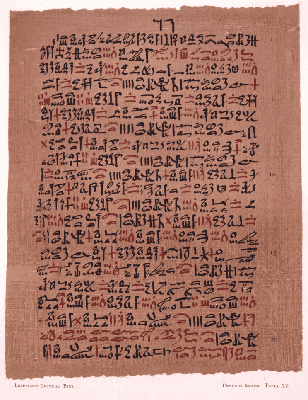
\includegraphics[width=\columnwidth]{Papyrus_Ebers.png}}
		\small{Écriture \href{https://en.wikipedia.org/wiki/Hieratic}{hiératique}, égypte ancienne}
	\end{minipage}
\end{frame}

\begin{frame}
	\frametitle{Approche pédagogique}
	\begin{itemize}
		\item Peu de solutions clé en main
		\item Il vous faudra \emph{comprendre}
		\item Chercher dans la documentation (liens fournis)
	\end{itemize}
	\begin{block}{Deux astuces importantes}
		\begin{itemize}
			\item Vous aurez \emph{presque} toutes les clés
			\item Posez des questions !
		\end{itemize}
	\end{block}
\end{frame}

\subsection{Évaluation}
\begin{frame}
	\frametitle{Implémentation sur applications illustratives}
	
	\begin{itemize}
		\item Implémentation des techniques sur une \emph{application illustrative}
		\item Une application ≠ par groupe : 3 ou 4 membres
		\item Chaque membre responsable d’au moins une classe persistante non triviale
		\item Ajout éventuel de classes artificielles pour implémentations requises (t.q. héritage)
	\end{itemize}
	\begin{block}{Demande}
		\begin{itemize}
			\item Implémentation au fur et à mesure, par chacun ou le groupe
			\item Je vous indiquerai les contenus et dates de remise
			\item Remise exclusivement par serveur git
		\end{itemize}
	\end{block}
\end{frame}

\begin{frame}
	\frametitle{Évaluation}
	\begin{block}{Contrôle continu}
		\begin{itemize}
			\item 50\%
			\item qualité du code concernant JDBC ou JPA en isolation
		\end{itemize}
	\end{block}
	\begin{block}{Soutenance}
		\begin{itemize}
			\item 50\%
			\item mise en œuvre adéquate des technologies dans l’application
			\item qualité de la présentation finale
			\item fonctionnalités
			\item qualité générale de l’application
		\end{itemize}
	\end{block}
	Possibilité de rendre l’application finale fin avril.
\end{frame}

\subsection{Plan}
\begin{frame}
	\frametitle{Plan}
	\begin{itemize}
		\item Cours 1 à 4 : Intro, git, Maven, JDBC, DAO
		\item Cours 2 : projet Eclipse / Maven ; init. JDBC avec BD H2
		\item Cours 3 : postgresql ; JDBC ; DAO
		\item Cours 4 : suite JDBC et DAO
		\item Cours 5 à 8 : JPA
	\end{itemize}
\end{frame}

\section{Git}
\subsection{Présentation}
\begin{frame}
	\frametitle{Git}
	\begin{itemize}
		\item Contrôle de version (VCS, SCM) : conserver l’historique
		\item Pour tous types de projet : code, images, présentations, article…
		\item VCS local, centralisé, distribué ? \pause
		\item Centralisé : seulement sur un serveur distant
		\item Distribué : copie locale et distante
		\item Git : distribué
	\end{itemize}
\end{frame}

\subsection{Commits}
\begin{frame}
	\frametitle{Commits et historique}
	\begin{itemize}
		\item Blob : capture d’un fichier à un moment donné
		\item Commit : identifié par un hash SHA-1
		\begin{itemize}
			\item Contient : structure de répertoires ; \emph{blobs} ; auteur…
		\end{itemize}
		\item Histoire : un DAG de \og{}commits\fg{}
	\end{itemize}
	{
		\centering
		\begin{tikzpicture}
			\path node[/Git/commit] (c1) {98C49C};
			\path (c1.east) ++ (\GitCommitSep, 0) node[anchor=west, /Git/commit] (c2) {34AC2} edge[->] (c1);
			\path (c2.east) ++ (\GitCommitSep, 6mm) node[anchor=west, /Git/commit] (c3N) {F30AB} edge[->] (c2);
			\path (c2.east) ++ (\GitCommitSep, -6mm) node[anchor=west, /Git/commit] (c3S) {C32AC} edge[->] (c2);
			\path (c2 -| c3N.east) ++ (\GitCommitSep, 0) node[anchor=west, /Git/commit] (c4) {175E3A} edge[->] (c3N) edge[->] (c3S);
		\end{tikzpicture}\par
	}
\end{frame}

\begin{frame}
	\frametitle{Work dir (WD)}
	\begin{itemize}
		\item Histoire conservée \emph{localement} dans \texttt{.git} à la racine du projet
		\item WD (\og{}work dir\fg{}) : version du projet (fichiers et sous-répert.)
		\item Interaction avec sous-rép. \texttt{.git} : \emph{uniquement} via outils git
	\end{itemize}
	\texttt{/root}
	\begin{itemize}
		\item[] \texttt{/.git}
		\item[] \texttt{/rép1}
		\begin{itemize}
			\item[] \texttt{/fich1}
		\end{itemize}\vspace{-0.8ex}
		\item[] \texttt{/fich2}
	\end{itemize}
\end{frame}

\begin{frame}
	\frametitle{Préparer un commit}
	\begin{minipage}[t]{0.33 \columnwidth}
		\textbf{Work dir}
		\begin{itemize}
%			\item[] \texttt{/.git}
			\item[] \texttt{/rép1}
			\begin{itemize}
				\item[] \texttt{/fich1}
			\end{itemize}\vspace{-0.8ex}
			\item[] \texttt{/fich2}
			\item[] \texttt{/fich3}
		\end{itemize}
	\end{minipage}%
	\begin{minipage}[t]{0.33 \columnwidth}
		\textbf{Index}
		\begin{itemize}
			\item[] \texttt{/rép1}
			\begin{itemize}
				\item[] \texttt{/fich1'}
			\end{itemize}\vspace{-0.8ex}
			\item[] \texttt{/fich2}
		\end{itemize}
	\end{minipage}%
	\begin{minipage}[t]{0.33 \columnwidth}
		\textbf{HEAD}
		\begin{itemize}
			\item[] \texttt{/rép1}
			\begin{itemize}
				\item[] \texttt{/fich1}
			\end{itemize}\vspace{-0.8ex}
			\item[] \texttt{/fich2'}
		\end{itemize}
	\end{minipage}
	\begin{itemize}
		\item \emph{Index} : changements à apporter au prochain commit
		\item \emph{HEAD} : commit d’où le work dir actuel est issu
		\item Initialisation nouveau répertoire ? \pause Index et HEAD vide \pause
		\item Juste après un commit ? \pause Index vide
	\end{itemize}
\end{frame}

\begin{frame}
	\frametitle{Préparer un commit : définitions}
%	\small
	\begin{minipage}[t]{0.33 \columnwidth}
		\textbf{Work dir}
		\begin{itemize}
%			\item[] \texttt{/.git}
			\item[] \texttt{/rép1}
			\begin{itemize}
				\item[] \texttt{/fich1}
			\end{itemize}\vspace{-0.8ex}
			\item[] \texttt{/fich2}
%			\item[] \texttt{/fich3}
		\end{itemize}
	\end{minipage}%
	\begin{minipage}[t]{0.33 \columnwidth}
		\textbf{Index}
		\begin{itemize}
			\item[] \texttt{/rép1}
			\begin{itemize}
				\item[] \texttt{/fich1'}
			\end{itemize}\vspace{-0.8ex}
			\item[] \texttt{/fich2}
		\end{itemize}
	\end{minipage}%
	\begin{minipage}[t]{0.33 \columnwidth}
		\textbf{HEAD}
		\begin{itemize}
			\item[] \texttt{/rép1}
			\begin{itemize}
				\item[] %\texttt{/fich1}
			\end{itemize}\vspace{-0.8ex}
			\item[] \texttt{/fich2'}
		\end{itemize}
	\end{minipage}
	\begin{block}{Définitions (étant donné un fichier)}
	%nb on devrait peut-être appliquer modified et unmodified seulement pour les \emph{tracked}. Auquel cas on peut aussi définir :\item[\emph{modified}] [{∈} index ⇒ ≠ index] ; [{∉} index ⇒ {∈} HEAD ∧ ≠ HEAD]. Donc modified implique tracked.
		\begin{description}[\emph{unmodified}]
			\item[{∈} index] blob ds index, peut être ≠ WD
			\item[∈ HEAD] blob ds HEAD, peut être ≠ WD
			\item[\emph{untracked}] [{∉} index] et [{∉} HEAD]
			\item[\emph{tracked}] [{∈} index] ou [{∈} HEAD] {\tiny (ou les deux)}
			\item[\emph{modified}] [{∈} index ⇒ ≠ index] ; [{∉} index ⇒ ≠ HEAD]
			\item[\emph{unmodified}] [{∈} index ⇒ = index] ; [{∉} index ⇒ = HEAD]
		\end{description}
	\end{block}
\end{frame}

\begin{frame}
	\frametitle{Préparer un commit : commandes}
%	\begin{block}{Commandes}
		\begin{itemize}\setlength{\itemindent}{-1em}
			\item \texttt{git add fichier} : blob mis dans index (\og{}staged\fg{})
			\item \emph{clean} WD : tous {\tiny (sauf fichiers dans gitignore)} tracked et unmodified
			\item \texttt{git status} : liste untracked, {\tiny tracked-}modified, staged
			\item \texttt{git status -{}-short} {\tiny (sauf merge conflict)} : idx VS HEAD ; WD VS idx.
			\item \texttt{git diff} : WD VS index
			\item \texttt{git diff -{}-staged} : index VS HEAD
			\item \texttt{git commit} : commenter et expédier ! (Renvoie son id SHA-1)
			\item \texttt{git commit -v} : voir l’index en détail
		\end{itemize}
%	\end{block}
\end{frame}

\subsection{Branches}
\begin{frame}
	\frametitle{Branches et HEAD}
	\begin{itemize}
		\item Branche : pointeur vers un commit
		\item HEAD : pointeur vers {\tiny (typiquement)} une branche\\et un commit
		\item Branche \og{}actuelle\fg{}\\désignée par HEAD
	\end{itemize}
	\begin{tikzpicture}[overlay]
		\path (3.7cm, 0) node[/Git/commit] (c1) {98C49C};
		\path (c1.east) ++ (\GitCommitSep, 0) node[anchor=west, /Git/commit] (c2) {34AC2} edge[->] (c1);
		\path (c2.east) ++ (\GitCommitSep, 0) node[anchor=west, /Git/commit] (c3) {F30AB} edge[->] (c2);
		\path (c2.north) ++ (0, 3mm) node[anchor=south, /Git/branch] (master) {master} edge[->] (c2);
		\path (c3.north) ++ (0, 3mm) node[anchor=south, /Git/branch] (br) {br} edge[->] (c3);
		\path (br.north) ++ (0, 3mm) node[anchor=south, /Git/head] (head) {HEAD} edge[->] (br);
	\end{tikzpicture}
	\vspace{3mm}
	\begin{itemize}
		\item commit : avance HEAD et branche actuelle
		\item \texttt{git branch truc} : crée branche \texttt{truc}. HEAD inchangé !
		\item \texttt{git checkout truc} : change HEAD et met à jour WD
		\item Conseil : WD clean avant checkout !
		\item \texttt{git log -{}-graph -{}-decorate -{}-oneline -{}-all}
	\end{itemize}
\end{frame}

\begin{frame}
	\frametitle{Fusion de branches}
	{
	\centering
	\begin{tikzpicture}
		\path (3.7cm, 0) node[/Git/commit] (c1) {98C49C};
		\path (c1.east) ++ (\GitCommitSep, 0) node[anchor=west, /Git/commit] (c2) {34AC2} edge[->] (c1);
		\path (c2.east) ++ (\GitCommitSep, 4mm) node[anchor=west, /Git/commit] (c3N) {F30AB} edge[->] (c2);
		\path (c2.east) ++ (\GitCommitSep, -4mm) node[anchor=west, /Git/commit] (c3S) {C32AC} edge[->] (c2);
		\path (c2.north) ++ (0, 3mm) node[anchor=south, /Git/branch] (master) {master} edge[->] (c2);
		\path (c3N.north) ++ (0, 3mm) node[anchor=south, /Git/branch] (br) {br} edge[->] (c3N);
		\path (br.north) ++ (0, 3mm) node[anchor=south, /Git/head] (head) {HEAD} edge[->] (br);
	\end{tikzpicture}\par
	}
	\begin{itemize}
		\item \texttt{git merge autrebranche} : fusionne changements de \texttt{autrebranche} dans branche actuelle
		\item Si \texttt{autrebranche} est en avant de l’actuelle : \og{}fast-forward\fg{}
		\item Sinon, \og{}merge conflict\fg{} possible. Modifier les fichiers à la main et les ajouter à l’index puis commit pour créer un merge.
		\item checkout d’un commit {\tiny (ou tag)} sans branche {\tiny (detached head state)} : lecture !
	\end{itemize}
\end{frame}

\subsection{Serveurs distants}
\begin{frame}
	\frametitle{Serveurs distants}
	\vspace{-1pt}
	\begin{itemize}
		\item Réf. distante (\og{}remote ref\fg{}) : pointeurs vers branches {\tiny et tags} sur dépots distants
		\item \og{}Remote-tracking branch\fg{} : branche locale correspondant à une branche distante et qui connait l’état de la branche distante correspondante la dernière fois qu’on l’a vue
		\item Remote \og{}origin\fg{} supposé configuré ici
		\item \texttt{git branch -vv} : voir branches et correspondants distants
		\item \texttt{git fetch} : récupère les commits distants ; met à jour (ou crée) les références distantes
		\item \texttt{git push origin mabranche} : sinon, nouvelles branches restent locales
		\item \texttt{git remote show origin} : voir les réf. distantes
		\item Suivre une branche distante : checkout \texttt{origin/branche} ; créer branche locale ; \texttt{git branch -{}-set-upstream-to origin/branch}
	\end{itemize}
\end{frame}

\subsection{Divers}
\begin{frame}
	\frametitle{Divers}
	\vspace{-1pt}
	\begin{itemize}
		\item Utilisez gitignore {\tiny (\href{https://github.com/github/gitignore}{modèles})}
		\item Créez-vous une paire clé publique / privée
		\item Raccourcis : à éviter au début
		\item \texttt{git init} : dépôt vide dans rép. courant (rien n’est traqué)
		\item \texttt{git clone url} : cloner un dépôt (et non checkout !)
		\item \texttt{git stash} : WD $←$ HEAD
		\item \texttt{git tag -a montag} {\tiny (tag annoté, recommandé)} puis \texttt{git push origin montag}
		\item \texttt{git config -{}-global} : écrit dans \texttt{\textasciitilde/.gitconfig}
		\item Indiquez propriété \texttt{user.name} (et \texttt{user.email})
		\item Déterminer des \href{https://git-scm.com/book/en/v2/Git-Tools-Revision-Selection}{révisions} {\tiny exemple : HEAD\textasciicircum 1 pour parent de HEAD}
		\item \href{https://git-scm.com/book/en/v2/Git-Basics-Git-Aliases}{Alias}
		\item \href{https://git-scm.com/book/en/v2}{Documentation}
		\item GUI pour diff : \texttt{git difftool}
		\item GUI pour merge : \texttt{git mergetool}
	\end{itemize}
\end{frame}

\subsection{Références}
\begin{frame}
	\frametitle{Références}
	\begin{itemize}
		\item \href{https://git-scm.com/downloads}{Téléchargement} officiel
		\item \href{https://git-scm.com/book/}{Livre} Pro Git
		\item \href{https://try.github.io/}{tryGit}
	\end{itemize}
\end{frame}

\subsection{Exercices}
\begin{frame}[allowframebreaks]
	\small
	\frametitle{Exercices : Git}
	Git en local
	\begin{itemize}
		\item Définir globalement (au moins) \texttt{user.name}. Vérifier avec \texttt{git config -{}-list}.
		\item Créer un répertoire projet et dedans un fichier \texttt{début.txt} contenant \texttt{"coucou"}.
		\item Initialiser un dépôt git dans ce projet.
		\item Placer \texttt{début.txt} dans l’index. Modifier \texttt{début.txt} pour qu’il contienne \texttt{"coucou2"}. Visualiser la différence sur ce fichier entre la version WD, index, et dépôt. Faire en sorte que le blob dans l’index contienne bien \texttt{"coucou2"}.
		\item Effectuer un premier commit, qui contiendra uniquement \texttt{début.txt}. À l’issue de ce commit, vérifier que vous obtenez l’historique suivant.\par
		{
			\centering
			\begin{tikzpicture}
				\path node[/Git/commit] (c1) {C1};
				\path (c1.north) ++ (0, 3mm) node[anchor=south, /Git/branch] (master) {master} edge[->] (c1);
				\path (master.north) ++ (0, 3mm) node[anchor=south, /Git/head] (head) {HEAD} edge[->] (master);
			\end{tikzpicture}\par
		}
		\item Vous avez maintenant une idée audacieuse pour résoudre un problème dans votre projet. Comme vous n’êtes pas sûr de sa pertinence, vous désirez placer vos changements dans une nouvelle branche en attendant d’y réfléchir. Créer une branche \texttt{"dev"} ; y commettre un fichier \texttt{audacieux.txt} (en plus de \texttt{début.txt}, inchangé) contenant \texttt{"approche 1"}. Votre historique doit maintenant être celui-ci (vérifier !).\par
		{
			\centering
			\begin{tikzpicture}
				\path node[/Git/commit] (c1) {C1};
				\path (c1.north) ++ (0, 3mm) node[anchor=south, /Git/branch] (master) {master} edge[->] (c1);
				\path (c1.east) ++ (\GitCommitSep, 0) node[anchor=west, /Git/commit] (c2) {C2} edge[->] (c1);
				\path (c2.north) ++ (0, 3mm) node[anchor=south, /Git/branch] (dev) {dev} edge[->] (c2);
				\path (dev.north) ++ (0, 3mm) node[anchor=south, /Git/head] (head) {HEAD} edge[->] (dev);
			\end{tikzpicture}\par
		}
		\item À l’issue de ce travail harrassant, il vous vient une idée alternative. N’étant toujours pas sûr de la valeur de votre première idée (dans \texttt{dev}), vous repartirez de \texttt{master} pour l’implémenter. Depuis \texttt{master}, créer une branche \texttt{dev2}, et y commettre (en plus de \texttt{début.txt}, inchangé) un fichier \texttt{audacieux.txt} contenant \texttt{"approche alternative"}. Vérifier ensuite votre historique.\par
		{
			\centering
			\begin{tikzpicture}
				\path node[/Git/commit] (c1) {C1};
				\path (c1.north) ++ (0, 3mm) node[anchor=south, /Git/branch] (master) {master} edge[->] (c1);
				\path (c1.east) ++ (\GitCommitSep, 4mm) node[anchor=west, /Git/commit] (c2) {C2} edge[->] (c1);
				\path (c2.north) ++ (0, 2mm) node[anchor=south, /Git/branch] (dev) {dev} edge[->] (c2);
				\path (c1.east) ++ (\GitCommitSep, -4mm) node[anchor=west, /Git/commit] (c3) {C3} edge[->] (c1);
				\path (c3.south) ++ (0, -2mm) node[anchor=north, /Git/branch] (dev2) {dev2} edge[->] (c3);
				\path (dev2.south) ++ (0, -2mm) node[anchor=north, /Git/head] (head) {HEAD} edge[->] (dev2);
			\end{tikzpicture}\par
		}
		\item À la réflexion, votre première idée est bonne. L’intégrer dans \texttt{master} pour obtenir l’historique suivant. Prédire si vous obtiendrez un fast-forward et vérifier.\par
		{
			\centering
			\begin{tikzpicture}
				\path node[/Git/commit] (c1) {C1};
				\path (c1.east) ++ (\GitCommitSep, 4mm) node[anchor=west, /Git/commit] (c2) {C2} edge[->] (c1);
				\path (c2.north) ++ (0, 3mm) node[anchor=south, /Git/branch] (master) {master} edge[->] (c2);
				\path (master.west) ++ (-5mm, 0) node[anchor=east, /Git/branch] (dev) {dev} edge[->] (c2);
				\path (c1.east) ++ (\GitCommitSep, -4mm) node[anchor=west, /Git/commit] (c3) {C3} edge[->] (c1);
				\path (c3.south) ++ (0, -2mm) node[anchor=north, /Git/branch] (dev2) {dev2} edge[->] (c3);
				\path (master.north) ++ (0, 2mm) node[anchor=south, /Git/head] (head) {HEAD} edge[->] (master);
			\end{tikzpicture}\par
		}
		\item Tout bien réfléchi vous aimez également votre deuxième idée. L’intégrer à son tour dans \texttt{master} et obtenir cet historique. Quel problème allez-vous rencontrer, ce faisant ?\par
		{
			\centering
			\begin{tikzpicture}
				\path node[/Git/commit] (c1) {C1};
				\path (c1.east) ++ (\GitCommitSep, 4mm) node[anchor=west, /Git/commit] (c2) {C2} edge[->] (c1);
				\path (c1.east) ++ (\GitCommitSep, -4mm) node[anchor=west, /Git/commit] (c3) {C3} edge[->] (c1);
				\path (c1 -| c2.east) ++ (\GitCommitSep, 0) node[anchor=west, /Git/commit] (c4) {C4} edge[->] (c2) edge[->] (c3);
				\path (c4.north) ++ (0, 3mm) node[anchor=south, /Git/branch] (master) {master} edge[->] (c4);
				\path (master.north) ++ (0, 2mm) node[anchor=south, /Git/head] (head) {HEAD} edge[->] (master);
			\end{tikzpicture}\par
		}
		\item Imaginons qu’on aurait d’abord intégré \texttt{dev2} à \texttt{master} (ceci aurait-il produit un fast-forward ?) puis \texttt{dev} au résultat. Quel aurait été le résultat final ?
	\end{itemize}
	\framebreak
	Git distant
	\begin{itemize}
		\item Cloner votre dépôt central pour le projet de ce cours (ou votre dépôt local).
		\item Le clonage vous a créé un pointeur vers un serveur distant \texttt{origin}, et une \og{}remote-tracking branch\fg{} \texttt{master}. Voir où pointent \texttt{origin}, \texttt{master} et \texttt{origin/master}.
		\item Ajouter un fichier \texttt{"macontrib.txt"} contenant votre prénom à votre index local. Commettre dans votre dépôt git local. L’envoyer au dépôt distant. Vérifier (via l’interface web) qu’il s’y trouve et que le commit est associé à votre nom.
		\item Quand un collègue a fait de même, vous pouvez rapatrier sa modification en local. Après l’avoir fait, prédire où vont pointer \texttt{master} et \texttt{origin/master} et vérifier.
		\item Si un collègue a publié sa modification avant la vôtre, quel va être votre problème ? Comment le résoudre ? Si vous êtes le premier à publier la modification, allez aider vos collègues à publier la leur !
	\end{itemize}
\end{frame}

\section{Maven}
\subsection{Présentation}
\begin{frame}
	\frametitle{Présentation}
	\begin{itemize}
		\item Apache Maven
		\item Outil de gestion de projet
		\item Principalement gestion de dépendances
		\item Description de votre projet via POM (Project Object Model)
		\item Convention over configuration : peu de configuration grâce aux valeurs par défaut
		\item Dépôt central avec publications open source
		\item Fortement basé sur plugins
	\end{itemize}
\end{frame}

\begin{frame}[fragile]
	\frametitle{Le POM}
	\begin{itemize}
		\item Fichier XML
		\item Décrit un projet ou module et comment le construire (\emph{build})
		\item Un projet \emph{peut} être composé de modules
	\end{itemize}
	\begin{block}{Exemple de POM}
		\begin{lstlisting}
<project xmlns="http://maven.apache.org/POM/4.0.0"
 xmlns:xsi="…"  xsi:schemaLocation="…">
  <modelVersion>4.0.0</modelVersion>
  <groupId>myGroupId</groupId>
  <artifactId>myArtifactId</artifactId>
  <version>0.0.1-SNAPSHOT</version>
</project>
		\end{lstlisting}
	\end{block}
\end{frame}

\begin{frame}
	\frametitle{Structure du projet}
	Structure déterminée {\tiny normalement} par \emph{conventions}
	\vfill
	\begin{minipage}[t]{3.5cm}
%		\rule{\columnwidth}{1cm}
		{\centering Arborescence de base\par}
		\vspace{1ex}
		\texttt{pom.xml}\\
		\texttt{/src}
		\begin{itemize}
			\item[] \texttt{/main}
			\begin{itemize}
				\item[] \texttt{/java}
			\end{itemize}\vspace{-0.8ex}
			\begin{itemize}
				\item[] \texttt{/resources}
			\end{itemize}\vspace{-0.8ex}
			\item[] \texttt{/test}
			\begin{itemize}
				\item[] \texttt{/java}
			\end{itemize}\vspace{-0.8ex}
			\begin{itemize}
				\item[] \texttt{/resources}
			\end{itemize}\vspace{-0.8ex}
		\end{itemize}
	\end{minipage}\hfill%
	\begin{minipage}[t]{6.5cm}
		{\centering Répertoires de base\par}
		\begin{description}[\texttt{…/resources}]
			\item[\texttt{/src/main/…}] fichiers code et ressources \og{}normales\fg{}
			\item[\texttt{/src/test/…}] fichiers code et ressources pour tests
			\item[\texttt{…/java}] code java
			\item[\texttt{…/resources}] images, etc., devant être dans classpath
		\end{description}
	\end{minipage}
\end{frame}

\begin{frame}{Accès aux ressources en Java}
	Rappel : accès aux ressources en Java (indépendant de Maven)
	\begin{exampleblock}{Exemple d’accès aux ressources}
		\begin{itemize}
			\item \texttt{MyClass} dans package \texttt{com.mypkg}
			\item \texttt{URL url = MyClass.class.\href{https://docs.oracle.com/javase/8/docs/api/java/lang/Class.html\#getResource-java.lang.String-}{getResource}("ploum.txt")}
			\item \texttt{url} désigne la ressource de chemin \texttt{/com/mypkg/ploum.txt}
			\item Ensuite : \texttt{url.openStream()} (ou toute autre exploitation)
		\end{itemize}
	\end{exampleblock}
	\begin{block}{Positionnement de ressources avec Maven}
		Placer le fichier dans \texttt{/src/main/resources/com/mypkg/ploum.txt}
	\end{block}
\end{frame}

\subsection{Cycle de vie}
\begin{frame}
	\frametitle{Cycles de vie Maven}
	\begin{itemize}
		\item Maven utilise des cycles de vie
		\item Cycles embarqués : default ; clean ; site
		\item Cycle : ensemble ordonné de \emph{phases}
		\item Cycle “clean” contient {\tiny essentiellement} phase “clean”
		\item Cycle “site” contient {\tiny essentiellement} phase “site”
		\item Lors exécution de Maven, préciser une phase (Maven en déduit le cycle)
	\end{itemize}
\end{frame}

\begin{frame}{Cycle “default”}
	Phases {\tiny (non exhaustif)} dans cycle “default” :
	\begin{description}[process-resources]
		\item[validate] valide informations du projet
		\item[process-resources] copie vers destination
		\item[compile] compilation du code source
		\item[test] lancement des tests
		\item[package] création d’un paquet
		\item[integration-test] tests d’intégration
		\item[verify] vérification de la validité du paquet
		\item[install] installation en local
		\item[deploy] déploiement dans dépôt configuré
	\end{description}
\end{frame}

\begin{frame}
	\frametitle{Phases}
	\begin{itemize}
		\item Chaque phase associée à un ensemble de plugins et d’objectifs (\emph{goals})
		\item Phase process-resources associée {\tiny par défaut} à plugin \textbf{Resources}, objectif \texttt{resource}
		\item Phase test associée {\tiny par défaut} à plugin \textbf{Surefire}, objectif \texttt{test}
		\item Phase package associée {\tiny par exemple} à plugin \textbf{JAR}, objectif \texttt{JAR}
	\end{itemize}
	\begin{block}{Exécution}
		Lancement de Maven avec \texttt{mvn phasechoisie} :
		\begin{itemize}
			\item Maven détecte de quel cycle il s’agit
			\item Maven exécute toutes les phases jusqu’à “phasechoisie”
			\item Exemple : exécution systématique de \texttt{test} avant \texttt{package}
		\end{itemize}
	\end{block}
\end{frame}

\subsection{Dépendances}
\begin{frame}
	\frametitle{Dépendances}
	\begin{itemize}
		\item Maven permet de gérer les \og{}dépendances\fg{}
		\item Bibliothèques dont votre code dépend
		\item Pour compiler (dépendance statique) ; s’exécuter ; pour tests uniquement…
		\item Une bibliothèque dont vous dépendez peut elle-même avoir des dépendances
		\item Maven gère ces dépendances transitives pour vous !
		\item Dépendances prises {\tiny par défaut} dans Maven Central Repository
		\item Dans POM : section \texttt{<dependencies>}
		\item Dans cette section : ajouter une section \texttt{<dependency>} pour chaque dépendance à gérer
	\end{itemize}
\end{frame}

\begin{frame}[fragile]
	\frametitle{Dépendances : exemples}
	\begin{block}{Exemple : dépendance vers Google \href{https://github.com/google/guava/blob/master/README.md}{Guava}}
		\begin{lstlisting}
<dependency>
  <groupId>com.google.guava</groupId>
  <artifactId>guava</artifactId>
  <version>19.0</version>
</dependency>
		\end{lstlisting}	
	\end{block}
	\begin{block}{Exemple : dépendance vers junit}
		\begin{lstlisting}
<dependency>
  <groupId>junit</groupId>
  <artifactId>junit</artifactId>
  <version>4.12</version>
  <scope>test</scope>
</dependency>
		\end{lstlisting}	
	\end{block}
\end{frame}

\begin{frame}
	\frametitle{Dépendances dans POM}
	\begin{itemize}
		\item Trouver \texttt{groupId} et \texttt{artifactId} : voir site du projet
		\item Trouver \texttt{version} : voir \href{https://search.maven.org}{Central}
		\item Presque tous les projets Java récents font une release Maven
	\end{itemize}
	Portées {\tiny (liste non exhaustive)} :
	\begin{description}[\texttt{runtime}]
		\item[\texttt{compile}] Par défaut
		\item[\texttt{test}] Bibliothèque incluse uniquement lors phase tests
		\item[\texttt{runtime}] Bibliothèque incluse uniquement lors exécution, pas lors compilation
	\end{description}
\end{frame}

\subsection{Configuration}
\begin{frame}
	\frametitle{Configuration des plugins}
	\begin{itemize}
		\item Voir \href{https://maven.apache.org/plugins/index.html}{Liste} pour plugins de Apache
		\item Configuration parfois utile
		\item Dans POM : ajouter section \texttt{<build><plugins><plugin>…</plugin></plugins></build>}
		\item Exemple : pour configurer la compilation, voir la page “Apache Maven Compiler Plugin”
	\end{itemize}
\end{frame}

\begin{frame}[fragile]
	\frametitle{Propriétés}
	\begin{itemize}
		\item Propriété \texttt{ma propriété} : accessible via \texttt{\$\{ma propriété\}}
		\item Nommage souvent hiérarchique : \texttt{catégorie.sous-catégorie.nom-propriété}
	\end{itemize}
	Dans POM : 
	\begin{lstlisting}[keywordstyle=\fontspec{Latin Modern Mono Light}\textbf, emph={project, modelVersion, groupId, artifactId, version}, emphstyle=\fontspec{Latin Modern Mono Light}\textbf, language=XML, basicstyle=\small\NoAutoSpacing\ttfamily, aboveskip=0pt, belowskip=0pt, showstringspaces=false]
<properties>
  <cat.etc.prop1>valeur1</cat.etc.prop1>
  <cat.etc.prop2>valeur2</cat.etc.prop2>
</properties>
(...)
<balise-quelconque>${cat.etc.prop1}</balise-quelconque>
		\end{lstlisting}
\end{frame}

\subsection{En pratique}
\begin{frame}
	\frametitle{Conventions et configurations classiques}
	\begin{itemize}
		\item Utiliser comme groupeId un nom unique : généralement un nom de domaine inversé
		\item Le paquet de base de toutes les classes doit être ce nom
		\item Indiquer propriété \texttt{project.build.sourceEncoding} avec valeur \texttt{UTF-8}
		\item Configurer maven-compiler-plugin avec valeurs \texttt{source} et \texttt{target} à \texttt{1.8}
	\end{itemize}
\end{frame}

\begin{frame}
	\frametitle{Conventions pour ce cours}
	\begin{itemize}
		\item Utiliser \texttt{groupId} : \texttt{fr.dauphine.lamsade.hib.nomapp}
		\item Utiliser \texttt{artifactId} : \texttt{nomapp}
		\item Canevas simple disponible \href{https://github.com/oliviercailloux/jee/tree/master/Sample/pom.xml}{ici}
	\end{itemize}
\end{frame}

\begin{frame}
	\frametitle{Installation}
	\begin{itemize}
		\item Installer Java 1.8 pour ce cours
		\item Installer \href{https://www.eclipse.org/downloads/}{Eclipse IDE for Java EE Developers} : contient maven embarqué
		\item Facultatif : \href{https://maven.apache.org/download.cgi}{télécharger} et installer maven indépendant d’eclipse
	\end{itemize}
\end{frame}

\begin{frame}
	\frametitle{Maven et Eclipse}
	\begin{itemize}
		\item M2Eclipse (m2e) fournit support Maven pour Eclipse
		\item Maven embarqué
		\item Wizards pour démarrer ou importer un projet maven
		\item Conseil : utiliser l’option \texttt{Maven / Update project / Update project configuration from pom.xml} pour configuration correcte du projet dans Eclipse
	\end{itemize}
\end{frame}

\subsection{Références}
\begin{frame}
	\frametitle{Références}
	\begin{itemize}
		\item \href{https://maven.apache.org/guides/getting-started/index.html}{Tutoriel} Apache Maven
		\item \href{http://gen.lib.rus.ec/book/index.php?md5=6e0bc8159b52299fdb912e3726c43bd9}{Apache Maven Cookbook}, Raghuram Bharathan, 2015
	\end{itemize}
	Omis dans cette présentation :
	\begin{itemize}
		\item Archetypes (\href{http://maven.apache.org/archetype/maven-archetype-plugin/usage.html}{maven-archetype-plugin})
		\item Packaging
		\item Assembly (\href{http://maven.apache.org/plugins/maven-assembly-plugin/}{maven-assembly-plugin})
	\end{itemize}
\end{frame}

\section{JDBC}
\subsection{Présentation}
\begin{frame}
	\frametitle{Présentation}
	\begin{itemize}
		\item JDBC ? \pause Java Database Connectivity \pause
		\item Une API pour se connecter à des données relationnelles
	\end{itemize}
	\begin{minipage}[t]{4cm}
		\begin{itemize}
			\item Programmation indépendante du fournisseur de BD
			\item App. programmée via API JDBC
			\item App. inclut pilotes du fournisseur
			\item Ces pilotes font la traduction
		\end{itemize}
	\end{minipage}\hfill%
	\begin{minipage}[t]{6.6cm}
		\begin{tikzpicture}[baseline=(App.north)]
			\path node[draw, ellipse] (App) {Application};
			\path (App.south) ++(0, -3mm) node[draw, ellipse, anchor=north] (JDBC) {API JDBC};
			\path (JDBC.south) ++(-1.4cm, -3mm) node[draw, ellipse, anchor=north] (Driver1) {Pilote Pg.};
			\path (Driver1.south) ++(0, -6mm) node[draw, ellipse, anchor=north] (BD1) {BD Postgresql};
			\path (JDBC.south) ++(1.4cm, -3mm) node[draw, ellipse, anchor=north] (Driver2) {Pilote H2};
			\path (Driver2.south) ++(0, -2mm) node[draw, ellipse, anchor=north] (BD2) {BD en mémoire};
			\path[<->, draw] (App) -- (JDBC);
			\path[<->, draw] (JDBC) -- (Driver1);
			\path[<->, draw] (JDBC) -- (Driver2);
			\path[<->, draw] (Driver1) -- (BD1);
			\path[<->, draw] (Driver2) -- (BD2);
		\end{tikzpicture}
	\end{minipage}
\end{frame}

\subsection{Instanciation}
\begin{frame}
	\frametitle{Instantiation}
	\begin{itemize}
		\item Souhait : instancier pilote adéquat avec minimum de code spécifique à un fournisseur
		\item API JDBC nous fournit \jseref{java.sql/DriverManager}
		\item Appeler \texttt{DriverManager.getConnection(String url)}
		\item \texttt{url} au format \texttt{jdbc:subprotocol:subname}
		\item Exemple : \texttt{jdbc:postgresql:mydb} (cf. \href{https://jdbc.postgresql.org/documentation/head/connect.html}{Doc JDBC Postgresql})
	\end{itemize}
	Mais comment ça marche ?
\end{frame}

\begin{frame}
	\frametitle{Fonctionnement de l’instantiation}
	\begin{itemize}
		\item Le pilote fournisseur est inclus aux bibliothèques runtime de l’application
		\item Le JAR pilote inclut un fichier nommé (par convention) \texttt{META-INF/services/java.sql.Driver}
		\item Ce fichier nomme la classe que \texttt{DriverManager} doit charger
		\item \texttt{DriverManager} charge toutes ces classes (si plusieurs pilotes accessibles)
		\item Ayant l’URL, \texttt{DriverManager} cherche un pilote enregistré qui peut la lire
		\item Il instancie ce pilote et le renvoie à l’appelant ou l’utilise en arrière-plan
	\end{itemize}
	
\end{frame}

\begin{frame}
	\frametitle{Remarques concernant l’instanciation}
	\begin{itemize}
		\item Avec \texttt{DriverManager} on peut aussi obtenir le \jseref{java.sql/Driver} (utile pour avoir n° de version par exemple)
		\item Beaucoup de tutoriels sur le net suggèrent d’enregistrer explicitement le pilote {\tiny par exemple avec \texttt{Class.forName()}}. Ce n’est plus nécessaire depuis longtemps (cf. explication précédente).
	\end{itemize}
\end{frame}

\subsection{Exercices}
\begin{frame}%[allowframebreaks]
	\frametitle{Exercices JDBC}
	Objectif : accéder à une BD en mémoire, à l’aide de H2
	\begin{itemize}
		\item Créer un projet Maven dans eclipse
		\item Indiquer H2 comme dépendance (cf. site \href{http://www.h2database.com}{H2})
		\item Bien choisir la portée de votre dépendance
		\item Trouver l’URL JDBC à laquelle vous connecter (cf. site)
		\item Faites un simple \texttt{main} dans lequel vous vous connectez au pilote via JDBC et obtenez le numéro de version
	\end{itemize}
\end{frame}

\section{Logging}
\subsection{Introduction}
\begin{frame}
	\frametitle{Utilité du logging}
	Logging : pour quoi faire ? \pause
	\begin{itemize}
		\item Débug pour soi-même
		\item Écriture systématique de ce qui se passe : souhait de conserver les informations dans le code
		\item Tout en pouvant désactiver la sortie à la demande
		\item Gain de temps possible par rapport à points d’arrêt
		\item Débug chez le client
		\item Visualisation des opérations des bibliothèques utilisées
		\item Granularité fine : seulement tel type de message
		\item Exemple : voir les commandes SQL envoyées par fournisseur de persistance
	\end{itemize}
\end{frame}

\begin{frame}
	\frametitle{Moteurs de logging}
	\begin{itemize}
		\item Ici : utilisation de Java util logging (JUL)
		\item Partie de Java SE
		\item En Java SE comme en Java EE
		\item Autres moteurs populaires de logging en Java : SLF4J, Commons logging {\tiny voir \hyperlink{Bataille}{annexe} pour brève justification du choix}
		\item Interfaçage {\tiny généralement presque} transparent
		\item Exemple : Hibernate utilise JBoss Logging, mais fonctionne avec logging standard
	\end{itemize}
\end{frame}

\begin{frame}
	\frametitle{Vue d’ensemble}
	\begin{itemize}
		\item Développeur utilise \jseref{java.util.logging/Logger}s pour logger
		\item Relation parent – enfant d’après noms des loggers
		\item Loggers passent les logs {\tiny sous forme de \jseref{java.util.logging/LogRecord}s} à \jseref{java.util.logging/Handler}
		\item Passés aussi à logger parent
		\item \texttt{Handler}s publient (avec \jseref{java.util.logging/Formatter}s)
		\item Ou \texttt{Handler} fait suivre à autre \texttt{Handler}
		\item \texttt{Logger}s et \texttt{Handler}s utilisent log levels et filtres
	\end{itemize}
	\begin{tikzpicture}
		\path node[/logger/main] (logger) {logger};
		\path (logger.east) ++ (1cm, 0) node[/logger/main, anchor=west] (handler) {handler};
		\path[->, draw] (logger) -- (handler);
		\path (handler.east) ++ (1cm, 0) node[/logger/main, anchor=west] (handler2) {handler2};
		\path[->, draw] (handler) -- (handler2);
		\path (handler2.east) ++ (1cm, 0) node[/logger/main, anchor=west] (out) {monde extérieur};
		\path[->, draw] (handler2) -- (out);
		\path (logger.north) ++ (0, 3mm) node[/logger/main, anchor=south] (logger parent) {logger parent};
		\path[->, draw] (logger) -- (logger parent);
		\path (handler2.south) ++(3mm, -6mm) node[/logger/helper, anchor=north west] (formatter) {formatter};
		\path[/logger/helper line] (formatter) -- (handler2);
		\path (handler2.south) ++ (-3mm, -6mm) node[/logger/helper, anchor=north east] (filterh2) {filtre handler2};
		\path[/logger/helper line] (filterh2) -- (handler2);
		\path (logger.south) ++ (0, -6mm) node[/logger/helper, anchor=north] (filterl) {filtre logger};
		\path[/logger/helper line] (filterl) -- (logger);
	\end{tikzpicture}
\end{frame}

\subsection{Loggers}
\begin{frame}
	\frametitle{Hiérarchie}
	\begin{itemize}
		\item Root logger nommé ""
		\item Hiérarchie suit typiquement le nom des packages
		\item Recommandation : nommer le logger d’une classe selon le nom de la classe
	\end{itemize}
	\begin{tikzpicture}
		\path[level distance=1.2cm, level 2/.style={sibling distance=5cm}, level 3/.style={sibling distance=3.2cm}] node {""}
			child {
				node {"app"}
					child {
						node {"app.pack1"}
							child {
								node {"app.pack1.MyClass"} 
							}
					}
					child {
						node {"app.pack2"} 
							child {
								node {"app.pack2.Class2"} 
							}
							child {
								node {"app.pack2.Class3"} 
							}
					}
			}
		;
	\end{tikzpicture}
\end{frame}

\begin{frame}[fragile]
	\frametitle{Obtention d’un \texttt{Logger}}
	\begin{itemize}
		\item Recommandation : \texttt{Logger} pour une classe stocké dans champ \texttt{private static Logger logger}
		\item Obtenir logger d’après nom avec \texttt{Logger.getLogger(String)}
		\item Nom : \texttt{MyClass.\href{https://docs.oracle.com/javase/8/docs/api/java/lang/Class.html}{class}.getCanonicalName())}
		\item String renvoyé ? \pause "app.pack1.MyClass" \pause
		\item Avantage par rapport à  \texttt{Logger.getLogger("app.pack1.MyClass")} ? \pause Refactoring : nom lié explicitement à la classe \pause
	\end{itemize}
	\begin{lstlisting}
private static Logger logger = Logger.getLogger(
    MyClass.class.getCanonicalName());
	\end{lstlisting}
\end{frame}

\subsection{Mise en œuvre}
\begin{frame}
	\frametitle{Loggons}
	\begin{itemize}
		\item Recommandation : se concentrer sur 3 niveaux de log {\tiny (parmi \href{https://docs.oracle.com/javase/8/docs/api/java/util/logging/Level.html}{sept})}
		\item SEVERE (erreurs), INFO, FINE (debug fin)
		\item \texttt{logger.info(String)}
		\item \texttt{logger.log(Level, String, Throwable)}
		\item \texttt{logger.log(Level, String, Object[])}
		\item Ne pas logger une exception si elle est relancée (pourquoi ? \pause sinon, double log !)
	\end{itemize}
\end{frame}

\begin{frame}
	\frametitle{Configuration}
	\begin{itemize}
		\item \jseref{java.util.logging/LogManager} chargé de la configuration
		\item \texttt{LogManager} est singleton
		\item Lit fichier de configuration au démarrage {\tiny ou utilise classe spéciale}
		\item D’après propriété système \texttt{java.util.logging.config.file}
		\item Format standard fichier de propriétés java {\tiny (\jseref{java.util/Properties})}
		\item Sinon, configuration par défaut {\tiny fichier \texttt{lib/logging.properties} installé avec Java}
		\item Aussi possible configurer via API de \texttt{LogManager}
	\end{itemize}
\end{frame}

\begin{frame}
	\frametitle{Fichier de configuration}
	Fichier de configuration contient des paires \texttt{prop = valeur}.\\
	Propriétés :
	\begin{description}[monlogger.useParentHandlers]
		\item[monlogger.level] Niveau de log de monlogger et ses enfants (cf. \jseref{java.util.logging/Level})
		\item[monlogger.handlers] Liste de classes \texttt{Handler}s pour monlogger
		\item[handlers] Liste de classes \texttt{Handler}s pour root logger
		\item[monlogger.useParentHandlers] Bool, indique s’il faut faire suivre le message aux parents
		\item[HandlerClass.level] Niveau de log de HandlerClass
		\item[HandlerClass.prop] Autre propriété de HandlerClass
	\end{description}
\end{frame}

\begin{frame}
	\frametitle{Handlers et formatters inclus}
	Handlers inclus :
	\begin{description}[\jseref{java.util.logging/ConsoleHandler}]
		\item[\jseref{java.util.logging/StreamHandler}] Écrit dans un OutputStream
		\item[\jseref{java.util.logging/ConsoleHandler}] Écrit dans \texttt{System.err}
		\item[\jseref{java.util.logging/FileHandler}] Écrit dans fichiers
		\item[\jseref{java.util.logging/SocketHandler}] Écrit sur ports TCP
		\item[\jseref{java.util.logging/MemoryHandler}] Enregistre en mémoire
	\end{description}
	Formatters inclus :
	\begin{description}[\jseref{java.util.logging/SimpleFormatter}]
		\item[\jseref{java.util.logging/SimpleFormatter}]
		\item[\jseref{java.util.logging/XMLFormatter}]
	\end{description}
\end{frame}

\begin{frame}[fragile]
	\frametitle{Configuration : recommandations}
	\begin{itemize}
		\item Indiquer configuration dans un fichier \texttt{logging.properties}
		\item Livrer ce fichier avec l’application {\tiny (dans classpath : requiert un chargement adapté)}
		\item Permet à l’utilisateur de changer les options de log au besoin
		\item Indiquer à la JVM le fichier de configuration avec option \texttt{-Dprop=value}
		\item Changer le niveau de log de certains loggers en fonction intérêt du développeur
	\end{itemize}
	\begin{block}{Option JVM}
		\begin{itemize}
			\item Démarrer avec : {\small\texttt{"-Djava.util.logging.config.file=logging.properties"}}
			\item Dans eclipse : \texttt{Preferences / Java / Installed JREs / Edit / Default VM arguments}\vspace{-1pt}
		\end{itemize}
	\end{block}
	Exemple de configuration \href{https://github.com/oliviercailloux/jee/blob/master/Sample/logging.properties}{ici}
\end{frame}

\subsection{Références}
\begin{frame}
	\frametitle{Références}
	\begin{itemize}
		\item \href{https://docs.oracle.com/javase/8/docs/technotes/guides/logging/overview.html}{Guide} Oracle
	\end{itemize}
\end{frame}

\section{Applications}
\subsection{Instructions}
\begin{frame}
	\frametitle{Applications}
	\begin{itemize}
		\item Application multi-utilisateur
		\item En Java SE : simulé par multiples instances en parallèle
		\item OU Java EE (au choix)
		\item À gérer de façon agile car fonctionnalités ajoutées au fil du cours : cycles courts, refactoring…
		\item Fonctionnalités de l’application décrites de manière vague : à vous de compléter
		\item Fin d’année : présentation collective de vos applications
		\item Vote pour la meilleure application
	\end{itemize}
\end{frame}

\subsection{Applications possibles}
\begin{frame}
	\frametitle{Bd locale d’annonces intéressantes (ads)}
	
	\begin{itemize}
		\item Annonces collectées manuellement {\tiny ou automatiquement}
		\item Par exemple : recherche d’appartements, d’emploi
		\item Classement par attractivité subjective de chaque utilisateur
		\item Différents aspects à prendre en compte (taille appartement, proximité aux lieux d’intérêt, prix…)
		\item Utilité partielle associée à chaque aspect : un nombre entre $0$ et $1$
		\item Chaque utilisateur peut définir ses fonctions d’utilités partielles
		\item L’application montre les annonces attractives
	\end{itemize}
\end{frame}

\begin{frame}
	\frametitle{Gestion de biblio collaborative (biblio)}
	\begin{itemize}
		\item Solution à apporter : les bibliographies sont souvent incorrectes
		\item Entrées de bibliographies : livres ou musiques
		\item Chaque utilisateur peut commenter chaque entrée
		\item Chaque utilisateur peut confirmer ou informer les commentaires des autres
		\item Dès lors, un utilisateur a une réputation calculée
		\item Chaque utilisateur peut accorder sa confiance à d’autres utilisateurs (par priorité)
		\item L’application fournit donc une bibliographie personnalisée
	\end{itemize}
\end{frame}

\begin{frame}
	\frametitle{Définir et analyser des QCMs (mchoice)}
	\begin{itemize}
		\item Des enseignants peuvent définir des questions
		\item Des enseignants peuvent définir des réponses
		\item Des enseignants peuvent associer des points aux réponses ({≠} points pour ≠ enseignants)
		\item Un enseignant peut définir un QCM en choisissant des questions, des réponses, des coefficients
		\item Un enseignant peut définir un ensemble de questions à partir desquelles piocher des questions au hasard
		\item Un étudiant peut répondre au QCM
		\item Ou un groupe d’étudiants (points partagés pour le groupe)
		\item Un étudiant peut tenter de répondre seul ou demander de l’aide au groupe…
	\end{itemize}
\end{frame}

\begin{frame}
	\frametitle{Élection du meilleur projet (elections)}
	\begin{itemize}
		\item Un projet associé à un groupe de participants
		\item Un administrateur établit les règles de vote
		\item Chaque électeur (participant ou autre) peut voter pour un projet
		\item Ou ranger les projets
		\item L’administrateur peut interdire de voter pour son propre projet
		\item Option anonyme : l’identité des électeurs est oubliée
	\end{itemize}
\end{frame}

\begin{frame}
	\frametitle{Comparaison de prédictions météo (predictions)}
	\begin{itemize}
		\item Enregistrement des prédictions de différents sites
		\item Des utilisateurs indiquent la météo réelle
		\item Des utilisateurs peuvent confirmer les indications d’autres utilisateurs
		\item Calcul d’un degré de sincérité de chaque utilisateur
		\item Calcul de fiabilité des indications
		\item Calcul de fiabilité des prédictions
	\end{itemize}
\end{frame}

\section{À faire}
\begin{frame}
	\frametitle{À faire}
%	\footnotesize
	\begin{block}{À faire \emph{avant} le 3 mars}
		\begin{itemize}
			\item Enregistrez-vous chacun dans un groupe sur \href{https://mycourse.dauphine.fr/webapps/blackboard/execute/launcher?type=Course&id=_35222_1}{MyCourse}
			\item Min 3 membres, max 4 {\tiny (pour 3 projets)} (1\iers arrivés prioritaires)
			\item Nom groupe MyCourse = nom application = nom entre ()
			\item Créez un projet sur \href{https://github.com/}{GitHub} (ou \href{https://bitbucket.org/}{Bitbucket}) pour le groupe
			\item Nom projet git = nom application
			\item Ajoutez-moi à votre projet git
			\item Créez-vous chacun un compte sur le site en question
			\item Indiquez sur votre groupe MyCourse l’url git de votre projet
		\end{itemize}
	\end{block}
	\emph{Avant} le x signifie : avant qu’on soit le jour x. Donc au plus tard la veille à 23h59 + 1 minute.
\end{frame}

\begin{frame}
	\frametitle{À faire (suite)}
	\begin{block}{À faire \emph{avant} le 16 mars}
		\begin{itemize}
			\item Projet eclipse (configuration sur serveur git)
			\item Dépendance Maven : H2
			\item Le prg affiche le numéro de version du pilote, puis quitte
			\item À faire par chaque membre de chaque groupe
			\item Envoyez au git de votre groupe dans rép. \texttt{user.name}
		\end{itemize}
	\end{block}
\end{frame}

\begin{frame}
	\frametitle{Évaluation}
	\begin{itemize}
		\item Groupe ou individus notés sur échelle \{−{−}, {−}, N, +, ++\}
		\item Lire les commentaires sur My Course
		\item Commentaires pour tout le groupe : donnés seulement au premier nom du groupe
	\end{itemize}
\end{frame}

\begin{frame}
	\frametitle{Auteurs}
	Chaque commit doit pouvoir être associé à ses auteurs
	\begin{itemize}
		\item Choisir un nom d’utilisateur \alert{une fois pour toutes} et l’indiquer dans \texttt{user.name}
		\item Indiquer sur votre groupe MyCourse le lien entre identité réelle et \texttt{user.name} (si non évident)
		\item Je considère le vrai auteur comme celui indiqué par git
		\item Je tiens compte du reviewer éventuel
	\end{itemize}
	Pair programming apprécié
	\begin{itemize}
		\item Indiquez dans le commentaire du commit le binôme éventuel : \og\alert{reviewer: Machin}\fg avec Machin le \texttt{user.name}
		\item Mais chacun doit être auteur à part \sim{} égale
	\end{itemize}
\end{frame}

\appendix
\AtBeginSection{
}
\section{SLF4J – JUL}
\begin{frame}[label = Bataille]
	\frametitle{SLF4J – JUL}
	\begin{itemize}
		\item SLF4J souvent plébiscité sur le web comparé à JUL (\href{http://stackoverflow.com/questions/11359187/why-not-use-java-util-logging}{SO})
		\item Options toutes deux raisonnables, mais pour ce cours il fallait faire un choix : pourquoi JUL ?
		\item Favoriser les standards
		\item Fonctionne sans configuration dans environnement Java EE
		\item JUL \emph{semble} aussi populaire {\tiny d’après une estimation \emph{très} hasardeuse}
		\item On peut intégrer certains avantages de SLF4J \href{http://www.slf4j.org/legacy.html\#jul-to-slf4j}{après coup} {\tiny n’évite sans-doute pas une perte de performance, mais vraisemblablement sans importance}
	\end{itemize}
	\begin{block}{Popularité}
		\sisetup{round-mode=figures, round-precision=2, scientific-notation = engineering}
		Nombre de correspondances dans codes sur GitHub
		\begin{description}[SLF4J]
			\item[\href{https://github.com/search?l=java&q="org.slf4j"&type=Code}{SLF4J}] \num{1 639 253} {\tiny Ou \href{https://github.com/search?l=java&q="org.slf4j.Logger"&type=Code}{org.slf4j.Logger} : \num{1 604 000}}
			\item[\href{https://github.com/search?l=java&q="java.util.logging"&type=Code}{JUL}] \num{1 811 678} {\tiny Ou \href{https://github.com/search?l=java&q="java.util.logging.Logger"&type=Code}{java.util.logging.Logger} : \num{1495 000}}
		\end{description}
		{\tiny Mais il vaudrait mieux comparer le nombre de (gros) projets (récents) qui utilisent chaque moteur…}
	\end{block}
\end{frame}

\section{Licence}
\begin{frame}
	\frametitle{Licence}
	\begin{itemize}
		\item Cette présentation, et le code LaTeX associé, sont sous \href{http://opensource.org/licenses/MIT}{licence MIT}.
		\item Vous êtes libres de réutiliser des éléments de cette présentation, sous réserve de citer l’auteur.
		\item Le travail réutilisé est à attribuer à \href{http://www.lamsade.dauphine.fr/~ocailloux/}{Olivier Cailloux}, Université Paris-Dauphine.
	\end{itemize}
	\small{(Ceci ne couvre pas les images situées dans le répertoire \texttt{graphics}, dont je ne suis pas l’auteur.)}
\end{frame}
\end{document}
\begin{frame}
	\frametitle{}
	\begin{itemize}
		\item 
	\end{itemize}
	\begin{block}{}
		
	\end{block}
\end{frame}

\section{Bibliographie}
\begin{frame}[allowframebreaks]
	\frametitle{Bibliographie}
	\def\newblock{\hskip .11em plus .33em minus .07em}
% 	\bibliography{zotero}
\end{frame}

\section{Autres}
\begin{frame}
	\frametitle{}
	\begin{itemize}
		\item 
	\end{itemize}
	\begin{block}{}
		
	\end{block}
\end{frame}
\end{document}
